\documentclass[12pt,twoside,book]{article}
\usepackage{docmute}

\input{../settings}

\begin{document}

%%%%%%%%%%%%%%%%%%%%%%%%%%%%%%%%%%%%%%%%%%%%%%%%%%%%%%%%%%%%%%%%%%%%%%%%%%%%%%%
\section{WIMP as a dark matter}
\setcounter{equation}{0}
\label{sec:DM}
%%%%%%%%%%%%%%%%%%%%%%%%%%%%%%%%%%%%%%%%%%%%%%%%%%%%%%%%%%%%%%%%%%%%%%%%%%%%%%%

\vskip 0.1in

In this section, we review the properties of WIMPs as DM candidates.
It is revealed that, when we take a close look at the relic abundance of WIMP DM in Sec.~\ref{sec:relic}, a WIMP with the $\mathrm{TeV}$ scale mass is a good DM candidate, which is sometimes called \textit{WIMP miracle} and is a strong motivation to consider WIMPs.
In Sec.~\ref{sec:direct_detection} and \ref{sec:indirect_detection}, we will consider two different ways to search for WIMP DM, called the direct and indirect detection.
Finally, Sec.~\ref{sec:summary_DM} is devoted to the summary and concluding remarks of this section.


%%%%%%%%%%%%%%%%%%%%%%%%%%%%%%%%%%%%%%%%%%%%%%%%%%%%%%%%%%%%%%%%%%%%%%%%%%%%%%%
\subsection{WIMP DM relic abundance}
\label{sec:relic}
%%%%%%%%%%%%%%%%%%%%%%%%%%%%%%%%%%%%%%%%%%%%%%%%%%%%%%%%%%%%%%%%%%%%%%%%%%%%%%%

One of the most important evidence of the beyond SM phenomena is the existence of DM \cite{Zwicky:1933}.
DM is an unknown object that occupies a large fraction of the total energy of our universe but has not yet been directly observed because of its weak interaction with the SM particles.\footnote{
  At worst DM interacts with the SM particles through gravity, which is considerably weaker than all the other known interactions.
}
In spite of its invisibility, the existence of DM is confirmed by several astrophysical observations such as the mass measurement using the gravitational lensing effect caused by galaxies and clusters \cite{Zwicky:1937, Trimble:1987ee}, the flatness of galactic rotation curves further the optical radius \cite{1939LicOB..19...41B, Begeman:1991iy}, the measurement of the power spectrum of the cosmic microwave background (CMB), and so on.
In particular, the observation of CMB allows us the precise determination of various cosmological parameters \cite{Jungman:1995av, Jungman:1995bz} including the normalized density of the non-relativistic matter $\Omega_m$ and that of baryon $\Omega_b$, which is currently determined as \cite{Aghanim:2018eyx}
\begin{align}
  \Omega_m h^2 &= 0.1430 \pm 0.0011,\\
  \Omega_b h^2 &= 0.02237 \pm 0.00015,
\end{align}
where $h \sim \mathcal{O}(1)$ is the Hubble constant in units of $100\, \mathrm{km}\, \mathrm{s}^{-1}\, \mathrm{Mpc}^{-1}$.
The difference between $\Omega_m h^2$ and $\Omega_b h^2$ implies the existence of DM and its abundance $\Omega_\chi h^2 \simeq 0.12$.

In cosmology, DM production mechanisms that explain the DM abundance are divided into two large categories: thermal and non-thermal production.
The former assumes the equilibrium between the DM and the thermal bath in the early universe.
As the universe expands, the interaction rate that maintains the thermal equilibrium becomes smaller and the DM decouples from the thermal bath at some time, which is the so-called \textit{freezeout}.
As we will see below, the resulting abundance of the DM in this scenario is mainly controlled by the temperature of the thermal bath $T_f$ when the freezeout occurs.
On the other hand, non-thermal production assumes the DM production by some processes irrespective of the thermal bath such as the decay of a heavy particle.
From now on, we mainly focus on the case only with the thermal production, which gives the smallest possible relic abundance for WIMPs that have an interaction with the thermal bath through the electroweak interaction.

We assume the stable DM particle $\chi$ with mass $m_\chi$ that pair annihilates into SM particles with some cross section $\sigma$.
When DM is in thermal equilibrium with the thermal bath of temperature $T$, DM velocity obeys the corresponding Boltzmann distribution.
Let $v$ be the relative velocity of annihilating DM particles and $\Braket{\sigma v}$ be the thermal average of the product of $\sigma$ and $v$.
By using this quantity, we can write down the Boltzmann equation for the DM number density $n_\chi$ as
\begin{align}
  \frac{d (n_\chi a^3)}{d t} =
  - a^3 \Braket{\sigma v} (n_\chi^2 - n_{\mathrm{eq}}^2),\label{eq_boltzmann}
\end{align}
where $t$ and $a$ are the time coordinate and the scale factor, respectively, of the Friedmann Robertson Walker metric
\begin{align}
  d s^2 = - d t^2 + a(t)^2 d \bm{x}^2,
\end{align}
while $n_{\mathrm{eq}}$ denotes the number density of DM in equilibrium.
When DMs are non-relativistic, its temperature dependence is given by $n_{\mathrm{eq}} \propto T^{3/2} \exp \left( -m_\chi / T \right)$.
The first term of the right-handed side of Eq.~\eqref{eq_boltzmann} represents the annihilation rate of DM pairs that should be proportional to $n_\chi^2$, while the second term describes the DM creation through the inverse process.
As desired, the number density does not change in time if $n_\chi = n_{\mathrm{eq}}$.  Recalling the total entropy conservation in a comoving volume $s a^3 = (\mathrm{const})$, it turns out to be convenient to define the ratio $Y \equiv n_\chi / s$.
In fact, this modification cancels the effect of the expansion of the universe $da / dt > 0$ from Eq.~\eqref{eq_boltzmann}, leading to a simpler equation
\begin{align}
  \frac{d Y}{d t} =
  -s \Braket{\sigma v} (Y^2 - Y_{\mathrm{eq}}^2),\label{eq_boltzmann_Yt}
\end{align}
with $Y_{\mathrm{eq}} \equiv n_{\mathrm{eq}} / s$.

Here, we assume that the freezeout occurs when the relativistic radiation dominates the total energy of the universe, which will be verified to be correct later.
In this case, we can derive $a \propto T^{-1}$ from the entropy conservation with $s \propto T^3$.
For the numerical calculation, we define a dimensionless parameter $x \equiv m_\chi / T$.
Then Eq.~\eqref{eq_boltzmann_Yt} can be rewritten as
\begin{align}
  \frac{x}{Y_{\mathrm{eq}}} \frac{d Y}{d x} =
  -\frac{\Gamma}{H} \left( \frac{Y^2}{Y_{\mathrm{eq}}^2} - 1 \right),\label{eq_boltzmann_Yx}
\end{align}
where $\Gamma$ denotes the DM interaction rate defined as
\begin{align}
  \Gamma &\equiv n_{\mathrm{eq}} \Braket{\sigma v}.\label{eq_lambda}
\end{align}

\begin{figure}[t]
  \centering
  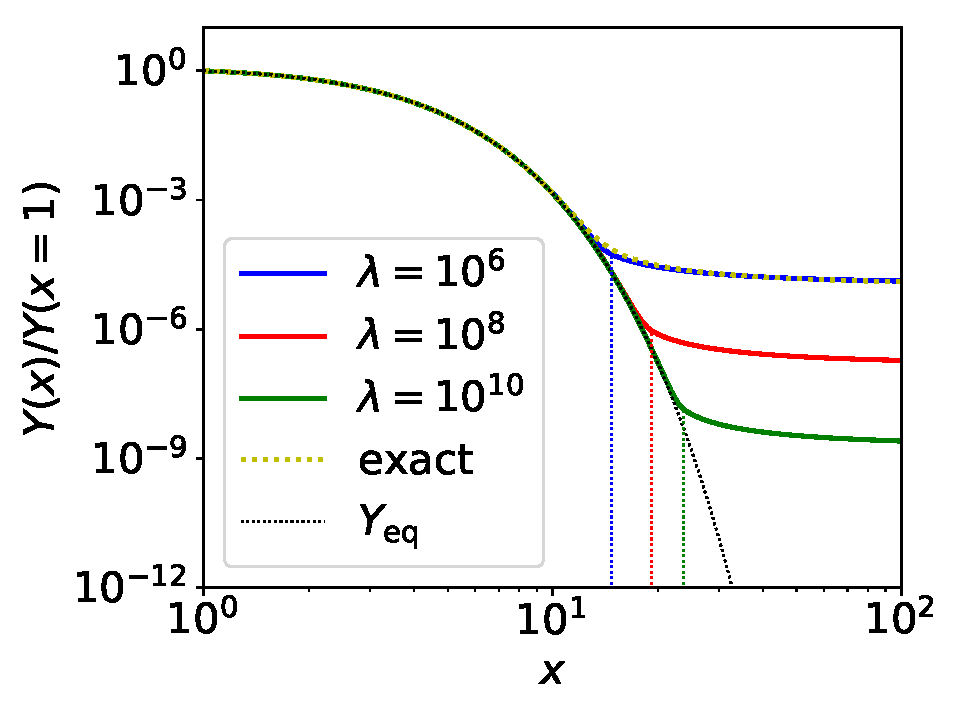
\includegraphics[width=0.5\hsize]{DMrelic.pdf}
  \caption{
    Plot of $Y(x) / Y(x=1)$ with $Y(x)$ being a solution of the evolution equation Eq.~\eqref{eq_boltzmann_Yx}.
    The yellow dotted line is a solution for $\lambda \equiv \left. \Gamma / H \right|_{x=1} = 10^6$, while the black dotted line denotes $Y_{\mathrm{eq}} (x) / Y_{\mathrm{eq}} (x=1)$.
    The solid lines are the approximation to the solutions described in the text.
    The blue, red, and green colors correspond to $\lambda = 10^8$, $10^{10}$, and $10^{12}$, respectively.
    The vertical dotted lines denote the freezeout temperature $x_f$.
  }
  \label{fig_DM_relic}
\end{figure}

Finally, $\Braket{\sigma v}$ is known to be expanded as~\cite{Gondolo:1990dk}
\begin{align}
  \Braket{\sigma v} = \Braket{\sigma v}_s +
  \Braket{\sigma v}_p x^{-1} + \cdots,
\end{align}
corresponding to the $s$-wave, $p$-wave, and so on, contributions to the cross section.
When $x \gg 1$, which is the same as the non-relativistic limit, the term with the highest power of $x$ dominates the cross section.  When the $x^{-p}$ term dominates ($p \geq 0$), the temperature dependence of the interaction rate is $\Gamma \propto x^{-3/2-p} e^{-x}$, while the Hubble parameter only reduces as $H \propto \rho^{1/2} \propto x^{-2}$.
As a result, at some point $\Gamma$ becomes smaller than $H$ and $Y$ freezes out as Eq.~\eqref{eq_boltzmann_Yx} indicates.
Hereafter, we focus on the case of the $s$-wave domination with $\Braket{\sigma v}_s \neq 0$ for simplicity.
\rem{Also comment on $p$-wave}
In Fig.~\ref{fig_DM_relic}, we show the solution of Eq.~\eqref{eq_boltzmann_Yx} for $\lambda \equiv \left. \Gamma / H \right|_{x=1} = 10^6$ by the yellow dotted line.
In the calculation, we use the boundary condition $Y(x=1) = Y_{\mathrm{eq}} (x=1)$ and plot the normalized value $Y(x) / Y(x=1)$.  We also plot the function $Y_{\mathrm{eq}} (x) / Y_{\mathrm{eq}} (x=1)$ by the black dotted line.

Unfortunately, it is computationally hard to solve Eq.~\eqref{eq_boltzmann_Yx} for larger values of $\lambda$ because of the almost complete cancellation between two terms of the right-handed side for small $x\sim \mathcal{O}(1)$ and its amplification caused by large $\lambda$.
We adopt instead to use an approximation that is the same as the one adopted in the public code \texttt{MicrOMEGAs}~\cite{Belanger:2001fz, Belanger:2018mqt}.
For the small $x$ region, temperature is still high enough to maintain the equilibrium $Y \simeq Y_{\mathrm{eq}}$, which means that $d \Delta Y / d x \ll d Y_{\mathrm{eq}} / d x$ with $\Delta Y \equiv Y - Y_{\mathrm{eq}}$.
From this approximation, we obtain a formula
\begin{align}
  \Delta Y \simeq -\frac{x}{2 \lambda} \frac{d Y_{\mathrm{eq}}}{d x}.\label{eq_relic_app_1}
\end{align}
Then we define the time $x_f$, or equivalently the so-called freezeout temperature $T_f$, when the approximation becomes invalid through the equation\footnote{
  One can easily check that the final relic abundance is not sensitive to the choice of the numerical coefficient $2.5$ in Eq.~\eqref{eq:freezeout_temperature}.
}
\begin{align}
  \Delta Y (x_f) = 2.5 Y_{\mathrm{eq}} (x_f).
  \label{eq:freezeout_temperature}
\end{align}
After the freezeout $x > x_f$, the annihilation of the DM pairs rapidly slows down and the DM abundance far exceeds its equilibrium value: $Y \gg Y_{\mathrm{eq}}$.
Then we can neglect the second term of the right-handed side of Eq.~\eqref{eq_boltzmann_Yx} and obtain the analytical solution
\begin{align}
  Y(x) \simeq - \frac{x}{c_1 x + \lambda / Y_{\mathrm{eq}} (x=1)},\label{eq_relic_app_2}
\end{align}
where $c_1$ is an integration constant.
In Fig.~\ref{fig_DM_relic}, we show results obtained with these two approximations Eqs.~\eqref{eq_relic_app_1} and \eqref{eq_relic_app_2} for $\lambda = 10^6$ (blue), $10^8$ (red), and $10^{10}$ (green).
In particular, the blue and the yellow lines almost completely overlap with each other, which proves the validity of the approximations.
The vertical dotted lines in the figure show the freezeout temperature.
It can be seen from the figure that $x = x_f$ does correspond to the time when $Y$ starts to deviate from $Y_{\mathrm{eq}}$.
Note also that as $\lambda \propto \Braket{\sigma v}$ becomes larger, the freezeout time becomes later and the resulting relic abundance becomes smaller.

When the DM properties (\textit{i.e.}, the mass $m_\chi$ and the annihilation cross section $\Braket{\sigma v}$ for a given temperature $T$) are given, corresponding relic abundance can be calculated using above procedure.
In particular, $m_\chi$ determines the normalization of the figure, namely $Y_{\mathrm{eq}} (x=1) = Y_{\mathrm{eq}} (T=m_\chi)$, and $\Braket{\sigma v}$ determines the freezeout temperature through the combination of Eq.~\eqref{eq_lambda}.
Assuming the absence of a non-thermal production, there should be a unique choice of $m_\chi$ corresponding to some $\Braket{\sigma v}$ to explain the current relic abundance of the DM.
From the numerical calculation, we obtain an order estimation formula
\begin{align}
  \Omega_\chi h^2 \sim \frac{3 \times 10^{-27}\,\mathrm{cm^3}/\mathrm{s}}
  {\Braket{\sigma v}_0} \sim
  0.1 \left( \frac{0.01}{\alpha} \right)^2
  \left( \frac{m_\chi}{300\,\mathrm{GeV}} \right)^2,\label{eq_relic_abundance}
\end{align}
where the rough estimation $\Braket{\sigma v} \sim \alpha^2/m_\chi^2$ is used in the last equation with $\alpha$ being the fine structure constant for the DM-SM coupling.
What is fascinating in Eq.~\eqref{eq_relic_abundance} is that a particle can be DM if it has a mass comparable to the electroweak scale and coupling constant comparable to the electroweak coupling constant.
This is the so-called \textit{WIMP miracle}, which supports the hypothesis of the WIMP as a candidate of the DM.
Such $\mathrm{TeV}$-scale WIMPs are theoretically well-motivated in connection with problems of the SM such as the naturalness problem as reviewed in Sec.~\ref{sec:model}.
Also, phenomenologically such $\mathrm{TeV}$-scale WIMPs are of great interest, since they can be detected using several different methods as will be described in this thesis.

In Table \ref{tab:WIMP_property}, we summarize the value of $m_\chi$ for each WIMP model that predicts the correct relic abundance $\Omega_\chi h^2 \sim 0.12$.
As described above, $\mathrm{TeV}$ scale masses are suitable for all WIMP DMs and the required mass becomes larger when we consider a larger $SU(2)_L$ $n$-plet because of the larger annihilation cross section.
However, note that the precise estimation of the relic abundance solely using the last term of Eq.~\eqref{eq_relic_abundance} is not possible, because of the so-called Sommerfeld enhancement effect \cite{Hisano:2004ds,Hisano:2006nn} that significantly modifies the annihilation cross section.
We will review this effect in more detail in Sec.~\ref{sec:indirect_detection} in relation to the indirect detection experiments.
Note also that $m_\chi$ in the table is only an upper bound on the WIMP DM mass because the existence of non-thermal production processes may allow lighter WIMPs to explain the whole relic abundance of DM in the current universe.


%%%%%%%%%%%%%%%%%%%%%%%%%%%%%%%%%%%%%%%%%%%%%%%%%%%%%%%%%%%%%%%%%%%%%%%%%%%%%%%
\subsection{WIMP DM search : direct detection}
\label{sec:direct_detection}
%%%%%%%%%%%%%%%%%%%%%%%%%%%%%%%%%%%%%%%%%%%%%%%%%%%%%%%%%%%%%%%%%%%%%%%%%%%%%%%

There are many experiments aimed at the direct detection of the DM\footnote
{
  For the recent review of the direct detection experiments, see for example \cite{Undagoitia:2015gya}.
}
proposed in \cite{Goodman:1984dc}.
Here, we assume some interaction between the DM and SM particles and look for the recoil of a target SM particle due to the collision with the DM in the laboratory.
In the case of WIMPs of our concern, any particle with non-zero electroweak charge can be a target particle, which interacts with WIMPs through the $t$-channel electroweak gauge boson exchange.
In the traditional setup such as the XENON1T experiment \cite{Aprile:2012zx}, a nucleus (of xenon in XENON1T) and an electron are the frequently used target particles.
From now on, we focus on the nucleus target since, as will be turned out later, it gives much better sensitivity than the electron target for DMs with a mass of $\mathcal{O} (\mathrm{TeV})$.
In this case, there are several ways to read out the information of the nuclear recoil depending on the deposited energy, such as the use of heat (or photons), an excitation of the nucleus associated with the emission of scintillation light, and the ionization of the atom.
Among them, the XENON1T experiment uses the scintillation light.

To evaluate the event rate for this kind of experiment, it is important to know the DM energy density $\rho_0$ and velocity distribution around us.
For this purpose, we model the DM profile in our galaxy using the so-called standard halo model (SHM) and adjust the parameters to the observations.
In the SHM, we assume the DM velocity distribution in the galactic rest frame
\begin{align}
  f(\bm{v}) = \frac{1}{\sqrt{2\pi \sigma}} \exp \left[ -\frac{\bm{v}^2}{2 \sigma^2} \right],
\end{align}
with $\sigma \equiv \sqrt{3/2} v_c$, where $v_c$ denotes the local circular speed of DMs around the galactic center.
From the combination of different analyses, we obtain the values $\rho_0 = 0.3\,\mathrm{GeV / cm^3}$ and $v_c = 220\,\mathrm{km/s}$ \cite{Kerr:1986hz,Green:2011bv}.
Also, the DM velocity within the halo cannot be arbitrarily large, since such energetic DM will not be gravitationally bound and will escape from our galaxy.
We often introduce a cutoff velocity $v_{\mathrm{esc}} = 544\,\mathrm{km / s}$ \cite{Smith:2006ym} and simply assume $f(\bm{v}) = 0$ for $|\bm{v}| > v_{\mathrm{esc}}$.

Using the distribution defined above, the differential event rate per unit recoil energy $E$ per unit material mass is given by \cite{Lewin:1995rx}
\begin{align}
  \frac{d R}{d E} (E,t) = \frac{\rho_0}{m_\chi m_T} \int d^3 v\, v f(\bm{v}, t)
  \frac{d \sigma}{d E} (E, v),
  \label{eq:rate}
\end{align}
where $m_T$ is the mass of the target nucleus, while $d\sigma / dE$ is the differential cross section of the DM-nucleus scattering.
The DM velocity distribution $f(\bm{v}, t)$ is now time-dependent since it represents the distribution observed at the laboratory, which is affected by the motion of the Earth around the Sun and that of the Sun around the galactic center.
Thus, $f(\bm{v}, t)$ is derived by performing the Galilean transformation to $f(\bm{v})$ according to the time-dependent velocity of the Earth against the galactic rest frame.
This time-dependence gives the signal a characteristic daily and yearly modulation, which helps us to distinguish it from the background events.
Also, the Galilean transformation makes $f(\bm{v}, t)$ highly anisotropic since the velocity of the Earth is comparable to $v_c$.
Thus, if it is possible to use the directional information, it also helps us to reduce the background.

The differential cross section $d\sigma / dE$, which summarizes the particle physics part of the calculation, is divided into two parts: the spin-independent (SI) part and the spin-dependent (SD) part.
Denoting the SI and SD scattering cross sections for zero momentum transfer as $\sigma_0^{\mathrm{SI}}$ and $\sigma_0^{\mathrm{SD}}$, respectively, we obtain
\begin{align}
  \frac{d\sigma}{d E} (E, v) = \frac{m_T}{2 \mu_T^2 v^2}
  \left( \sigma_0^{\mathrm{SI}} F_{\mathrm{SI}}^2 (E)
  + \sigma_0^{\mathrm{SD}} F_{\mathrm{SD}}^2 (E) \right),
\end{align}
with $\mu_T$ being the reduced mass of the WIMP-nucleus system.
The form factors $F_{\mathrm{SI}}$ and $F_{\mathrm{SD}}$ summarize the nuclear physics part of the matrix element, both of which have properties $F(0)=1$ and $dF / dE < 0$ for large $E$.
Among SI and SD contributions, the SI part is of great interest thanks to the possible coherent enhancement of the cross section.
When the de Broglie wavelength corresponding to the momentum transfer $q$ is longer than the size of the nucleus (corresponding to $q \lesssim 200\,\mathrm{MeV}$ for the xenon), not the individual neutrons and protons but the whole nucleus contribute to the cross section.\footnote{
  When the DM is lighter and the de Broglie wavelength is even longer, the collective excitation modes of nuclei or electrons such as the phonon becomes important.
  \rem{Reference}
  This corresponds to $q \lesssim \mathcal{O}(1)\,\mathrm{keV}$ or $m_\chi \lesssim \mathcal{O}(1)\,\mathrm{MeV}$ and thus we neglect this possibility here.
}
This results in the coherent contribution from all nucleons for the SI case, while only the unpaired nucleons contribute to the cross section for the SD case.
In fact, for the WIMP DM, the SI cross section $\sigma_0^{\mathrm{SI}}$ is originally non-zero and enhanced thanks to the coherence by a large factor $A$ that is the mass number of the target nucleus ($A \simeq 130$ for the xenon) as
\begin{align}
  \sigma_0^{\mathrm{SI}} = A^2 \sigma_p^{\mathrm{SI}} \frac{\mu_T^2}{\mu_p^2}
\end{align}
where $\sigma_p^{\mathrm{SI}}$ is the SI scattering cross section for a DM and a single nucleon and $\mu_p$ is the reduced mass of the WIMP-nucleon system.
The above expression dominates over the SD cross contribution for the WIMP DM.

\begin{figure}[t]
  \centering
  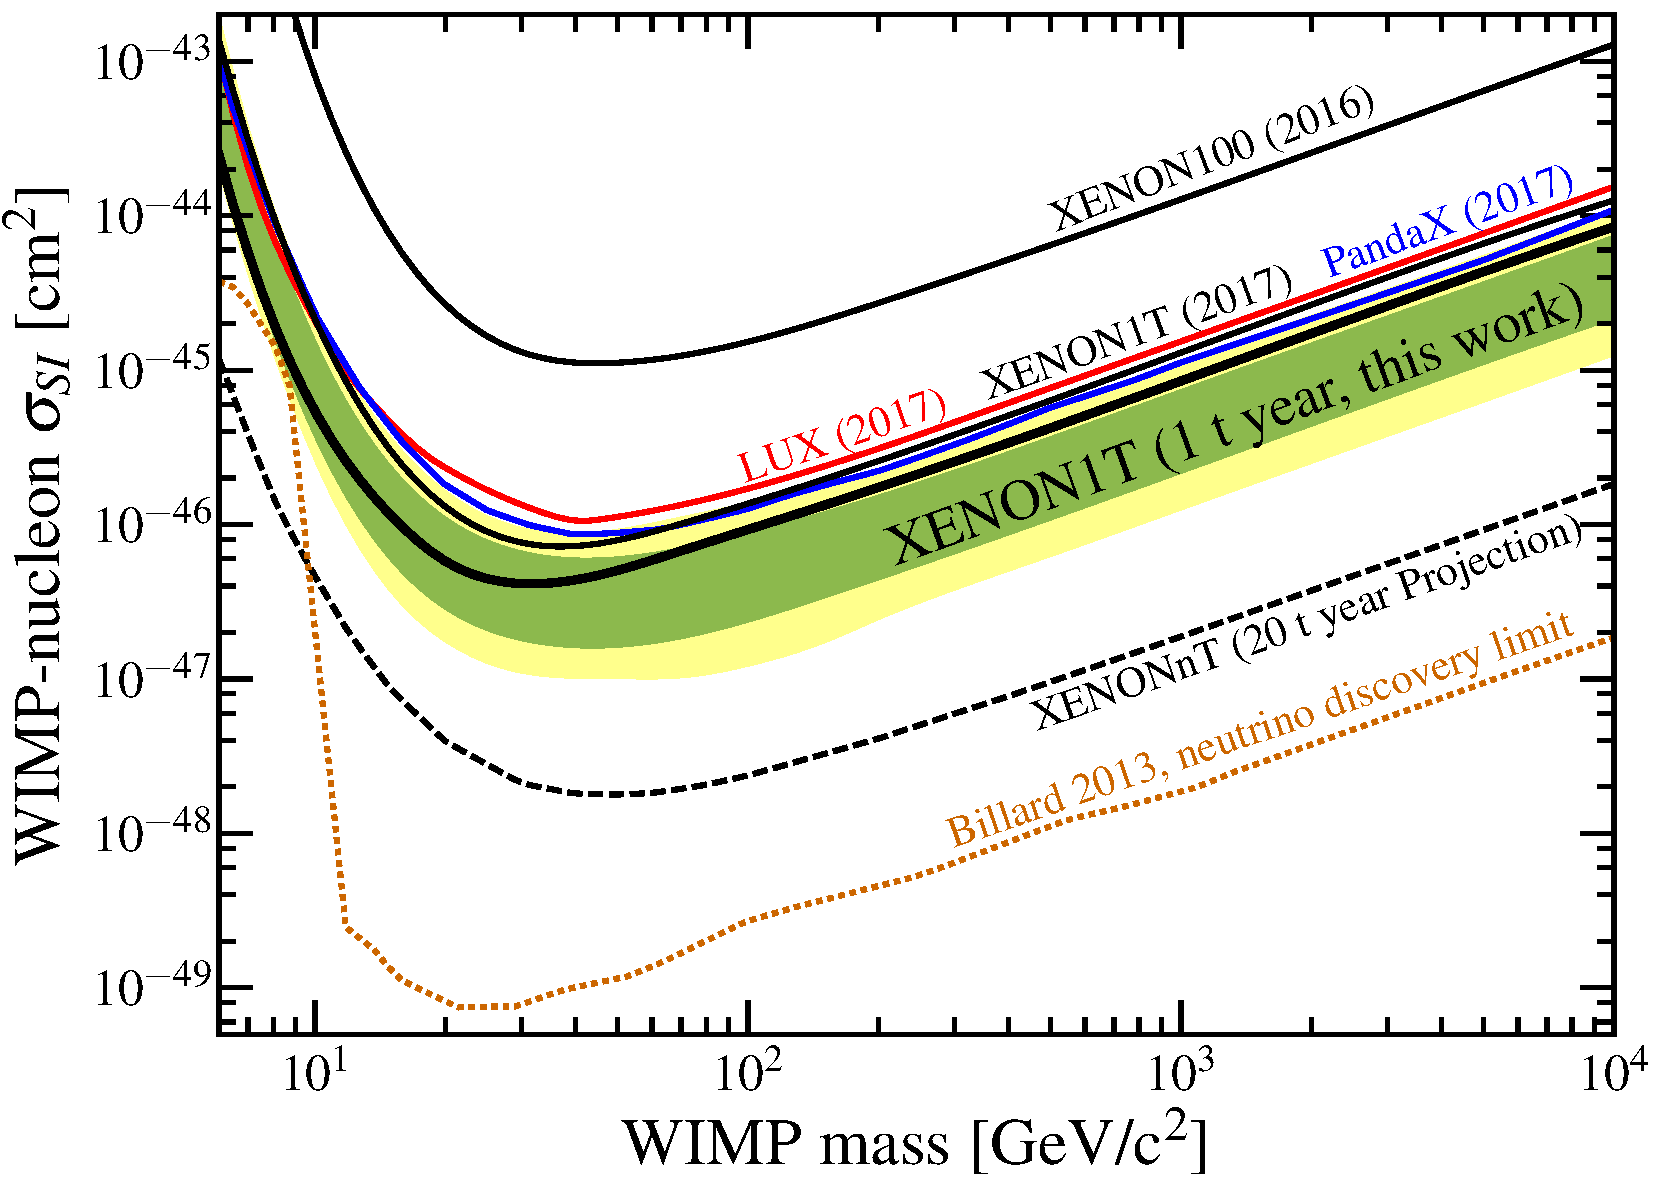
\includegraphics[width=0.5\hsize]{x1t_prelim_limits.pdf}
  \caption{
    Current constraint on the DM SI cross section taken from \cite{Aprile:2018dbl}.
    The $y$-axis corresponds to $\sigma_p^{\mathrm{SI}}$ in our notation.
  }
  \label{fig:XENON1T}
\end{figure}

In Fig.~\ref{fig:XENON1T}, we show the most recent constraint on the DM SI scattering cross section $\sigma_p^{\mathrm{SI}}$ as a function of its mass taken from \cite{Aprile:2018dbl} by the XENON1T collaboration.
The previous results of the LUX \cite{Akerib:2016vxi} and the PandaX-II \cite{Cui:2017nnn} experiments are also shown.
In the figure, the green and yellow bands represent the upper bound on the cross section with $1\sigma$ and $2\sigma$ experimental uncertainties, respectively.
Black dotted line corresponds to the prospect for the future experiment called XENONnT, while the orange dotted line represents the cross section of the background events sourced by neutrinos \cite{Billard:2013qya}.
This background often called as the neutrino floor, which is mainly determined by the solar neutrino for the region $m_\chi \lesssim 10\,\mathrm{GeV}$ and by the atmospheric and supernova neutrinos for $m_\chi \gtrsim 10\,\mathrm{GeV}$, roughly represents the maximum possible sensitivity of the direct detection method.\footnote{
  It may be possible, in particular for the solar neutrino background, to significantly reduce the number of background events and go beyond the neutrino floor by using the directional information of the signals.
}

The qualitative description of the form of the sensitivity curve in Fig.~\ref{fig:XENON1T} can be given using the above discussion.
The sensitivity for a very light WIMP is weak because of the finite threshold $E_{\mathrm{thr}}$ of the recoil energy required for the detection of the signal.
The threshold effect can be taken into account by choosing the lower boundary of the $\bm{v}$-integral in Eq.~\eqref{eq:rate} to be $v_{\mathrm{min}}$ defined as
\begin{align}
  v_{\mathrm{min}} = \sqrt{\frac{m_T E_{\mathrm{thr}}}{2 \mu_T^2}}.
\end{align}
Since $v_{\mathrm{min}} \propto m_\chi^{-1}$ for $m_\chi \ll m_T$, the event rate rapidly becomes smaller for smaller $m_\chi$.
On the other hand, heavier WIMPs have less number density with the energy density $\rho_0$ fixed.
Because of this, the sensitivity for a heavy WIMP becomes moderately worse when $m_\chi$ increases.
These two behaviors determine the best suitable $m_\chi$ for each choice of $m_T$ and $E_{\mathrm{thr}}$, which is the reason why the xenon nucleus target is more suitable for the $\mathrm{TeV}$-scale WIMP search than the electron target.
The latter choice is suitable when we search for lighter DMs.

Although no signal of DM is observed yet, this null result is still consistent with WIMP models of our concern.
For example, the calculation up to the next-to-leading order in $\alpha_s$ for the Wino DM reveals that the cross section almost mass-independently takes a small value of $\sigma_p^{\mathrm{SI}} \simeq 2.3 \times 10^{-47}\,\mathrm{cm}^2$~\cite{Hisano:2015rsa}, which is below the current constraint but is a region of future interest.
As for the MDM, the $5$-plet fermion is analyzed in \cite{Hisano:2011cs} and the scattering cross section $\sigma_p^{\mathrm{SI}} \simeq 10^{-46}\,\mathrm{cm}^2$ is obtained.
However, the mass requirement $m_\chi \sim 10\,\mathrm{TeV}$ (see Table~\ref{tab:WIMP_property}) makes the detection difficult and the sensitivity will not cover the whole region of the viable parameter space.
For Higgsino-like LSP, the constraint is highly model-dependent since the mixing between the Higgsino and Bino or Wino significantly modifies the scattering cross section.
According to \cite{Hisano:2012wm, Roszkowski:2014wqa}, the pure Higgsino has $\sigma_p^{\mathrm{SI}}$ below the neutrino floor, while some of the parameter space with a sizable mixing has much larger $\sigma_p^{\mathrm{SI}}$ that is already excluded.
Thus, we conclude that the almost pure Higgsino-like state is difficult to search for using this method.

\rem{Check constraints for $Y\neq 0$ MDM}


%%%%%%%%%%%%%%%%%%%%%%%%%%%%%%%%%%%%%%%%%%%%%%%%%%%%%%%%%%%%%%%%%%%%%%%%%%%%%%%
\subsection{WIMP DM search : indirect detection}
\label{sec:indirect_detection}
%%%%%%%%%%%%%%%%%%%%%%%%%%%%%%%%%%%%%%%%%%%%%%%%%%%%%%%%%%%%%%%%%%%%%%%%%%%%%%%

\rem{Briefly review later}

\rem{Sommerfeld enhancement}


%%%%%%%%%%%%%%%%%%%%%%%%%%%%%%%%%%%%%%%%%%%%%%%%%%%%%%%%%%%%%%%%%%%%%%%%%%%%%%%
\subsection{Summary}
\label{sec:summary_DM}
%%%%%%%%%%%%%%%%%%%%%%%%%%%%%%%%%%%%%%%%%%%%%%%%%%%%%%%%%%%%%%%%%%%%%%%%%%%%%%%

\rem{To search for WIMPs that do not compose a sizable fraction of the DM, we have to rely on the collider search.}


% \bibliographystyle{elsarticle-num}
% \bibliography{../phd}

\end{document}
